\documentclass[11pt]{article}

% set these commands
\newcommand{\course}{CSCI 534}
\newcommand{\proj}{Homework 04}
\newcommand{\dueDate}{3-18-2019}
\newcommand{\instructor}{David L. Millman}

\usepackage{../macros}

\begin{document}

\coverpage{04}

\newpage
\section*{Problem 1}

Draw a polygon with at least 4 vertices and give each vertex coordinates.
Using the duality discussed in class, draw the dual of the polygon.  In the
dual,
\begin{itemize}
    \item shade black the duals of the points that are on the vertices in the primal
    \item shade grey the duals of the points that are on the edges in the primal
    \item shade red the duals of the points that are inside the polygon in the primal
\end{itemize}

You should draw the primal and dual to scale.  You may draw the figure by hand,
but, I suggest using a tool like Ipe or Inkscape. \\\\

\answer
I ended up just using a drawing tool instead of Ipe or Inkscape because I was able to annotate the figure quite easily.

\begin{figure}[h]
    \centering
    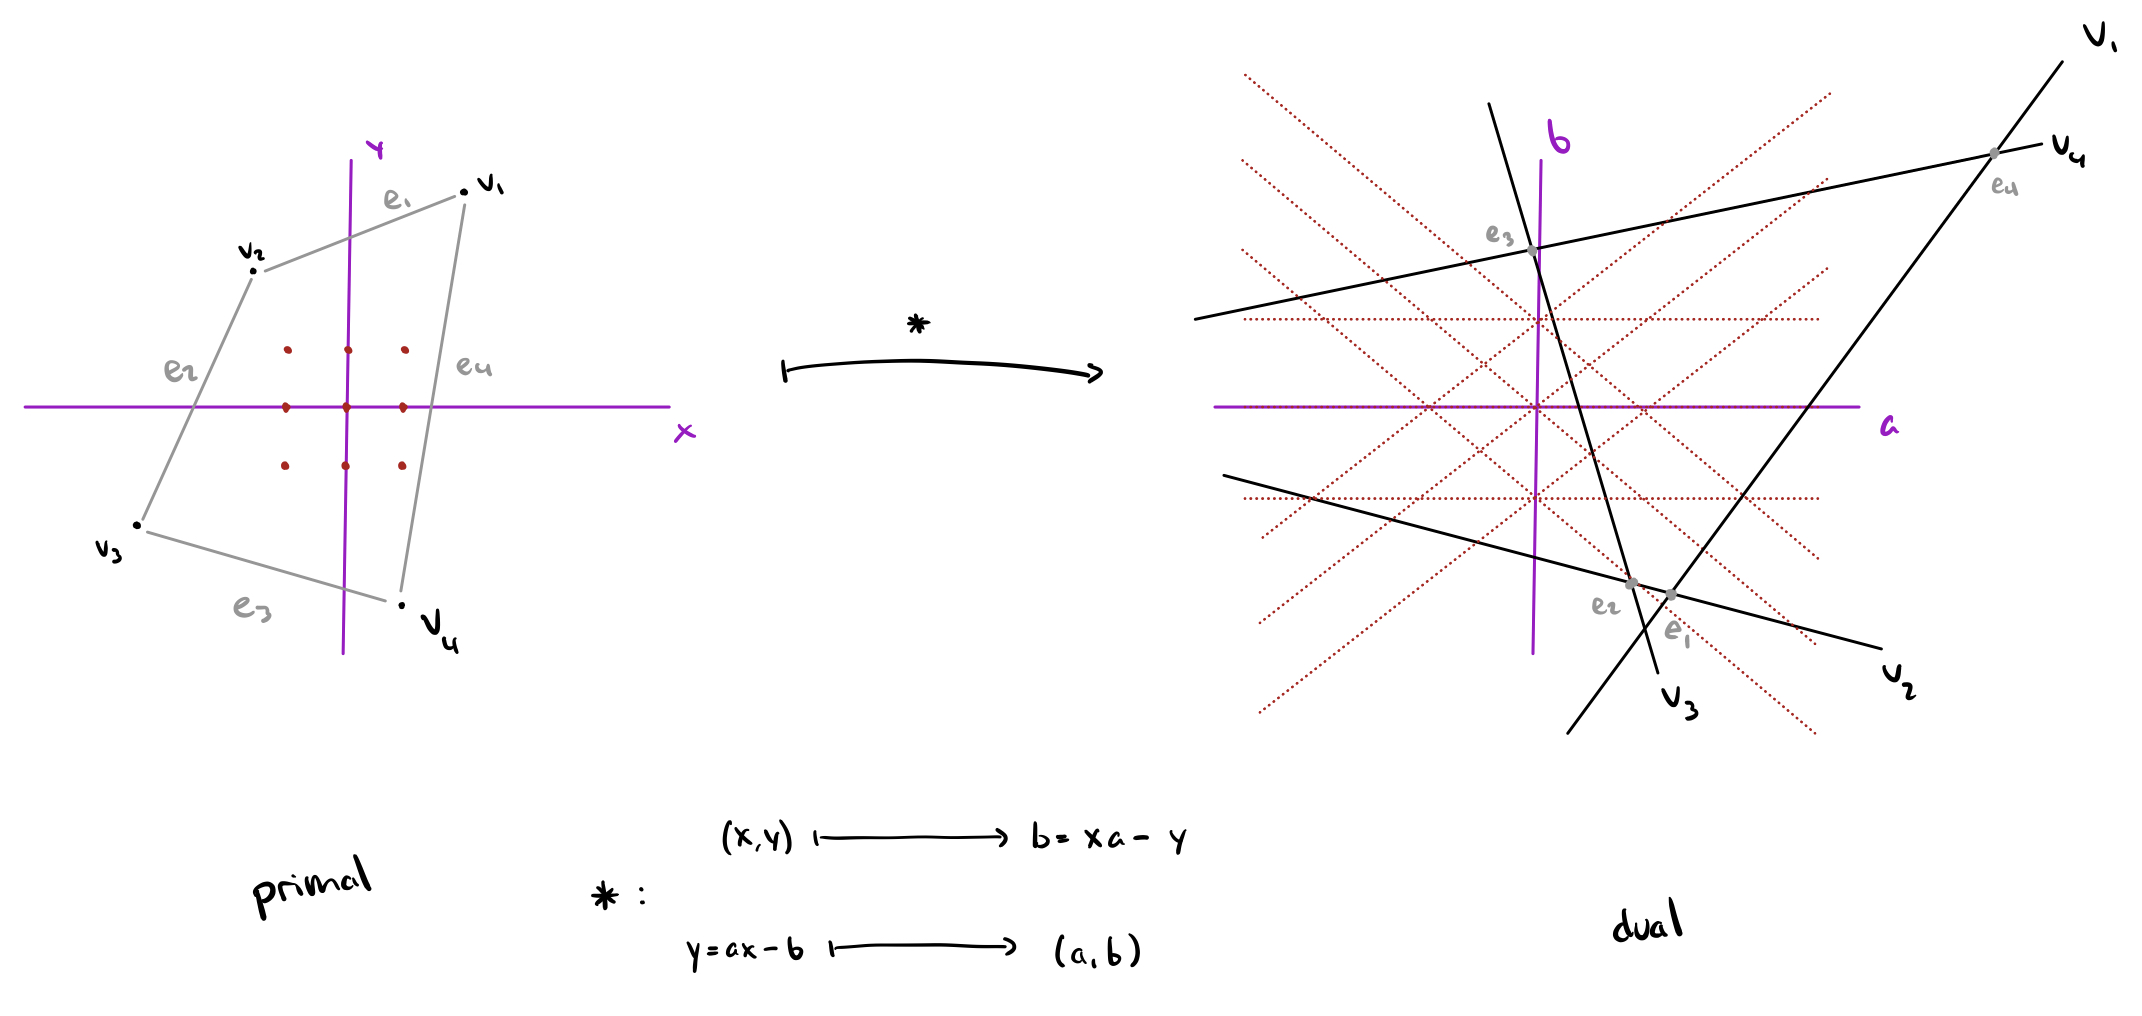
\includegraphics[width=0.95\textwidth]{polydual}
    \label{fig:polydual}
    \caption{Dual of a polygon with 4 vertices}
\end{figure}

In Figure 1, the left side is a polygon in the primal space and the right side is the dual of the polygon in the dual space.
Vertices in the primal are mapped to lines in the dual and edges are taken to points where the lines in the dual intersect.
I sampled 9 points inside the polygon and mapped them to their corresponding lines in the dual space.

\newpage
\section*{Problem 2}

Explain how to solve each of the following problems in linear (expected) time.
Each can be modeled as a linear programming (LP) problem, perhaps with some
additional pre- and/or post- processing. In each case, explain how the problem
is converted into an LP instance and how the answer to the LP instance is
used/interpreted to solve the stated problem.

\begin{enumerate}

    \item You are given two point sets $P = \{p_1,\ldots,p_n\}$ and $Q =
        \{q_1,\ldots,q_m\}$ in the plane, and you are told that they are
        separated by a vertical line $x = x_0$, with $P$ to the left and $Q$ to
        the right (see Fig. a). Compute the line equations of the two
        ``crossing tangents,'' that is, the lines $\ell_1$ and $\ell_2$ that are
        both supporting lines for $\rm{conv}(P)$ and $\rm{conv}(Q)$ such that
        $P$ lies below $\ell_1$ and above $\ell_2$ and the reverse holds for
        $Q$. (Note that you are not given the hulls, just the point sets.) Your
        algorithm should run in time $O(n + m)$.

    \begin{figure}[h]
        \centering
        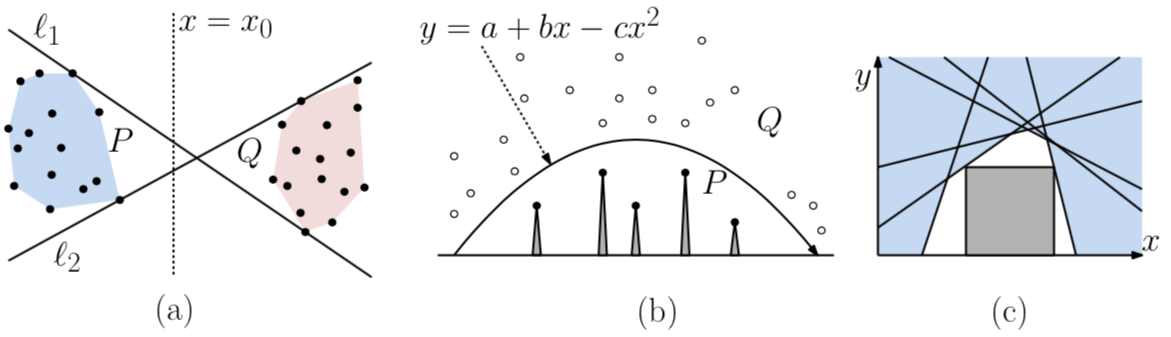
\includegraphics[width=0.75\textwidth]{lp}
        \label{fig:lp}
        \caption{Problem 3: LP applications}
    \end{figure}


    \item You have a cannon in $\R^2$. It has three controls labeled ``a'' ``b,''
        and ``c''. A projectile shot from this cannon travels along the
        parabolic arc $y = a + bx - cx^2$. You are asked to determine whether it
        is possible to adjust the controls so that the projectile travels above
        a set of $n$ building tops, represented by a point set $P = \{p_1,
        \ldots , p_n\}$ and beneath a set of $m$ floating balloons, represented
        by a point set $Q = \{q_1, \ldots , q_m\}$ (see Fig. b)). Your algorithm
        should run in time $O(n + m)$. (I do not care where the cannon is
        actually located. If your solution is based on some assumption about the
        cannon's location, please state this.)

    \item You are given a set of $n$ halfplanes $H = \{h_1,\ldots,h_n\}$, where
        $h_i$ is given as a pair $(a_i,b_i)$ and it consists of all the points
        of the plane that lie on or beneath the line $y = a_ix + b_i$. Compute
        the axis-parallel square of the largest side length whose lower edge
        lies on the x-axis (see Fig.~c). If no such square exists, your
        algorithm should indicate this.

\end{enumerate}

\answer
\begin{enumerate}

    \item We will provide an expected linear time algorithm to find the two crossing tangents by transforming this into a linear programming problem.
    That is, our goal is to transform the input into a set of intersecting halfplanes and an objective function.
    We will only describe the algorithm that finds $l_1$ since the algorithm that finds $l_2$ is only a minor modification.
    Note that the existence of the vertical line separating the two point sets guarantees that the two crossing lines exist.

    To transorm this problem into a linear programming problem, we use the dual map shown in Figure 3.
    That is, points in $P$ are taken to halfplanes above their defining line, points in $Q$ are taken to halfplanes below their defining line, and lines are just taken to the point $(a,b)$.

    \begin{figure}[h]
        \centering
        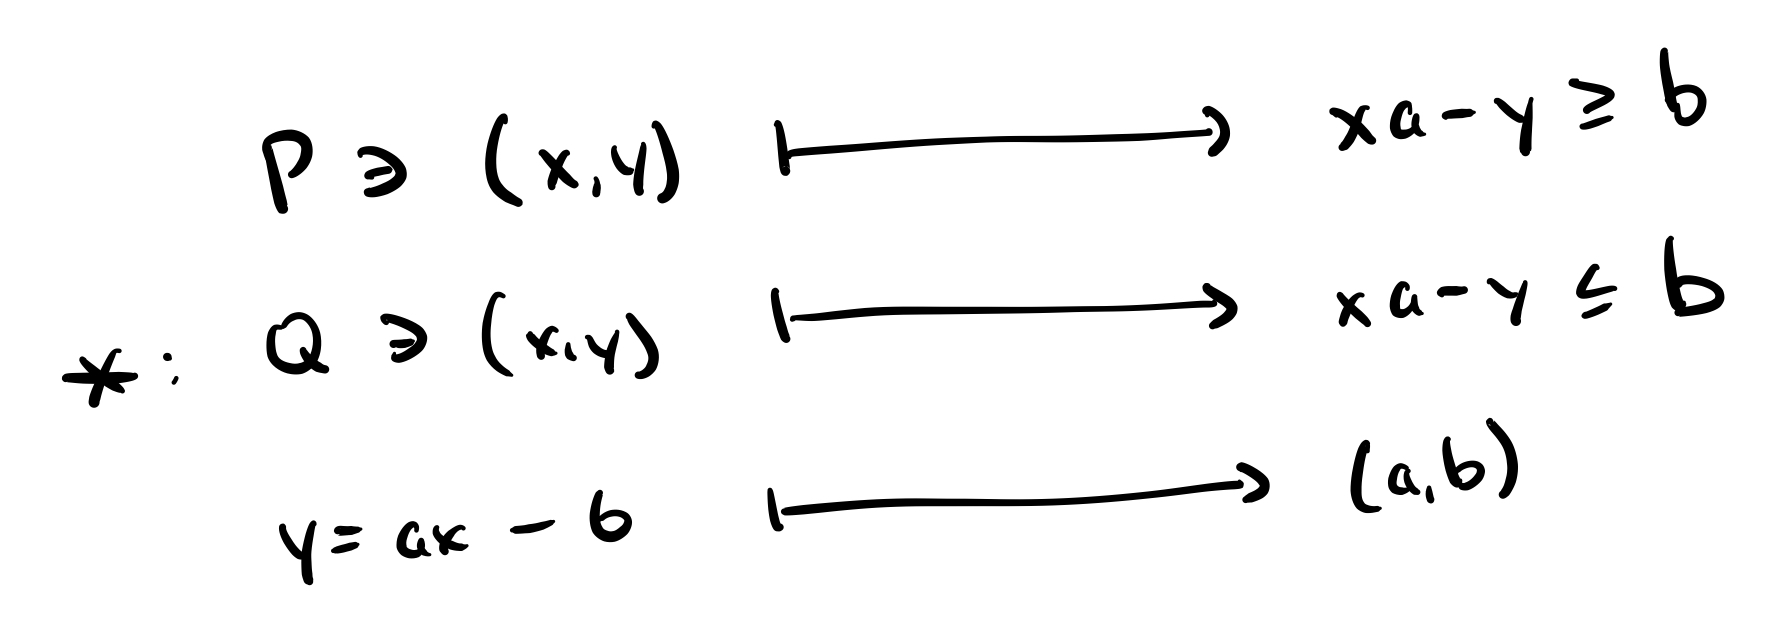
\includegraphics[width=0.5\textwidth]{dualpt1}
        \label{fig:dualpt1}
        \caption{Dual map for part 1}
    \end{figure}

    In the primal space, let $l$ be any line that satisfies the following over/under constraints.
    Evaluating $l$ at the $x$-coordinate of $p_i \in P$ must be greater than or equal to the $y$-coordinate of $p_i$ (in math: $l (p_i^x) \geq p_i^y$).
    And we must have $l (q_i^x) \leq q_i^y$ for all $q_i \in Q$ (note that $l_1$ satsifies these constraints).
    When we map to the dual, let $p_i^\star$ be the dual of the point $p_i \in P$, $q_i^\star$ be the dual of $q_i \in Q$, and $L = (L_x, L_y) \in \R ^2$ be the dual of $l$.
    Our constraints for $l$ turn into
    \begin{align}
        p_i^\star (L_x) = p_i^x * L_x - p_i^y \geq L_y &\iff p_i^x * L_x - L_y \geq p_i^y \\
        q_i^\star (L_x) = q_i^x * L_x - q_i^y \leq L_y &\iff q_i^x * L_x - L_y \leq q_i^y
    \end{align}
    Since $|P|=n$ and $|Q|=m$, this provides us with $n+m$ constraints that define a feasible region in $ab$ space.
    What is our objective function?
    Well, $l_1$ is the line with the largest slope that satisfies the over/under constraints for $P$ and $Q$.
    So our objective function is merely $L_x$.

    Now we have the necessary inputs for the linear programming algorithm which will run in expected $O(n+m)$ time and return a point in $\R ^2$.
    If we feed this point into the dual map, we get a line that is $l_1$!

    A quick note on runtime, we already know that the linear programming algorithm runs in expected $O(n+m)$ time but we must verify that reducing the input to a set of halfplanes also takes linear time.
    The reduction consists of turning each point into a line (an operation that takes $O(1)$ time).
    There are $n+m$ points so the reduction takes $(n+m) * O(1) = O(n+m)$ time.
    Thus the total run time is expected to be $O(n+m)$.

    \item This time we want to find the parabola that is below a certain set of points $Q$ but above another set of points $P$ in expected linear time.
    Linear programming is our friend again, let's just reduce the problem to a set of halfspace constraints!
    For this problem, any function will work for our objective function becuase we only want to know if the feasible region exists at all.

    Consider the map defined in Figure 4 which takes points to halfspaces in $\R ^2$ and parabolas to points in $\R ^3$.
    The parabola transformation is not super relevant for this problem, we only need to know that parabolas map to points in the same co-domain as the feasible region and that points in the feasible region map to parabolas in the primal.

    The meat of this map is the transformations on points.
    Let's justify the map, we will only justify the map for points in $P$ since the reasoning for points in $Q$ is analogous.
    For any point in $(u,v) \in P$, the parabola $f$ must satisfy $f(u) = a + bu - cu^2 \geq v$ (the parabola must be above the $v$-coordinate of the point).
    The reason $a + bu - cu^2$ traces a parabola is becuase $a,b,c \in \R$ are fixed and $u$ is varied over $\R$.
    If we were to instead fix $(u,v) \in \R^2$ and vary $(a,b,c) \in \R^3$ then we would have a halfspace $a + ub - u^2c \geq v$ in $\R^3$.
    Thus the condition that $f(u) \geq v$ and the halfplane $a + ub - u^2c$ evaluates to larger than $v$ are equivalent (they just represent different sets of solutions).
    This justifies our dual map.

    \begin{figure}[h]
        \centering
        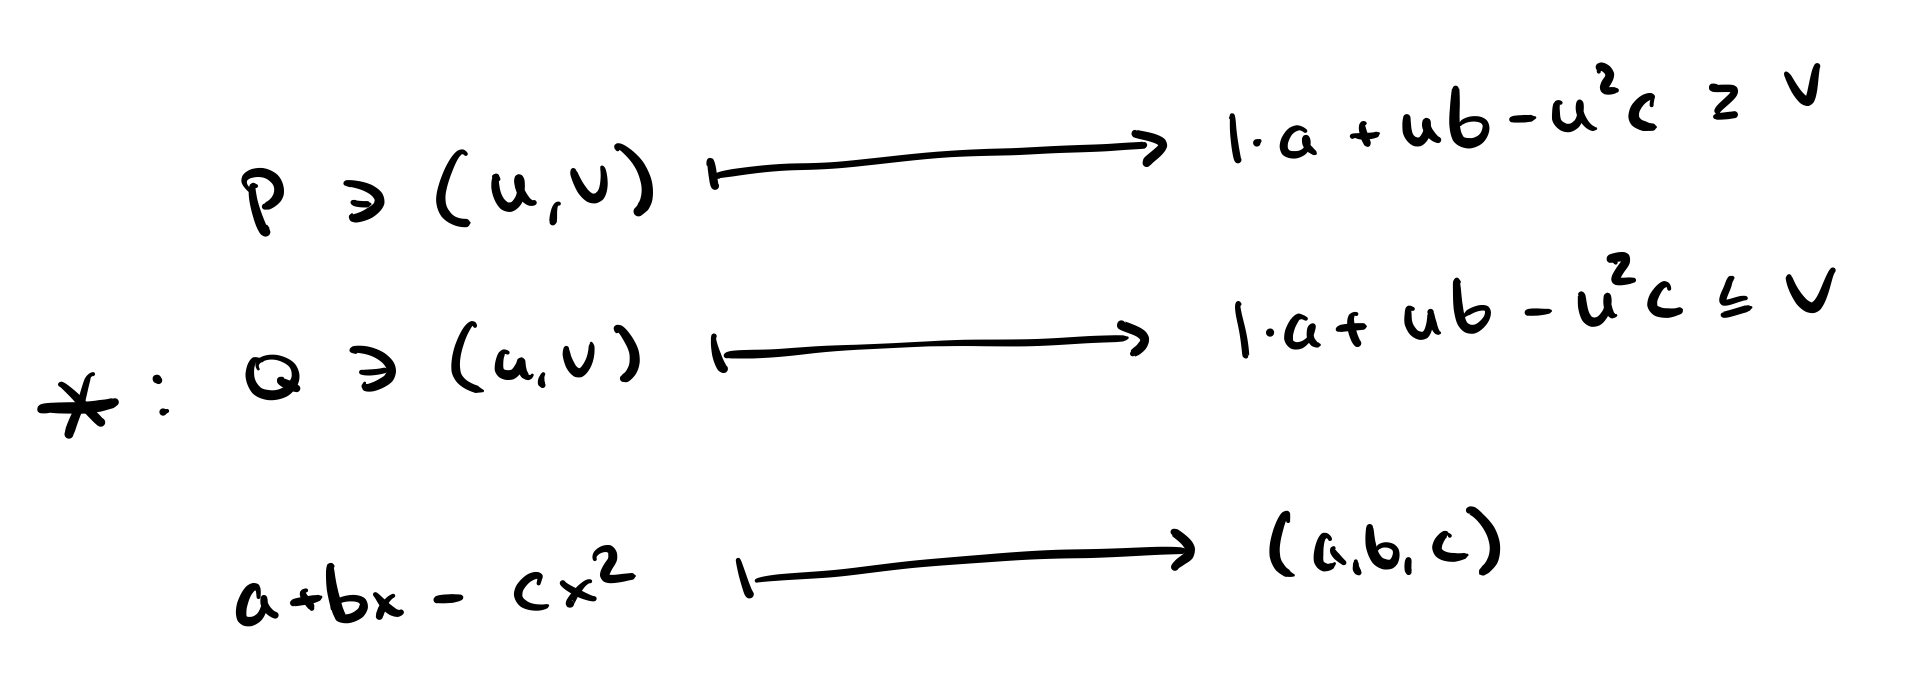
\includegraphics[width=0.55\textwidth]{dualpt2}
        \label{fig:dualpt2}
        \caption{Dual map for part 2}
    \end{figure}

    Since our dual map makes sense, we can apply the dual to each point in $P$ and $Q$ to obtain $n+m$ halfspace constraints in $\R ^3$.
    Then we can run the linear programming algorithm and return whether the feasible region exists or not.
    If someone wanted a parabola that satisifes the constraints, we could return any $(a,b,c)$ in the feasible region to represent the coefficeints of the parabola in the primal.

    What about the run time?
    As always, the linear programming will run in expected linear time in the number of constraints.
    There are $n+m$ constraints so we expect the linear programming portion to take $O(n+m)$ time.
    The reduction is a constant operation on $n+m$ items so the reduction takes $O(n+m)$ time.
    Thus the whole algorithm is expected to run in $O(n+m)$ time.

    \item Now we want to compute the largest square that lies above the x-axis and is in the intersection of the halfplanes $H = \{ h_1, \ldots, h_n \}$.
    Consider the square in Figure 5 which sits on the x-axis.
    The side length of the square is $r_x - l_x$, this is the objective function we wish to maximize.
    What are the constraints?
    We must have every point on the border of the square below every halfplane.
    Since the halfplanes have linear borders, this reduces to requring that the top corners on the left and right are below every halfplane.
    The height of the square is also $r_x - l_x$ so we must have
    $$ a_i*l_x + b_i \geq r_x - l_x \hspace{3em} a_i*r_x - b_i \geq r_x - l_x $$
    for every halfplane $h_i$.
    Since we are optimizing in $r_x, l_x$ space, let's rewrite the equations so the RHS is a constant.
    We require
    $$ r_x - (a_i + 1)*l_x \leq b_i \hspace{3em} -(a_i - 1)*r_x - l_x \leq b_i $$
    for all halfplanes $h_i$.

    \begin{figure}[h]
        \centering
        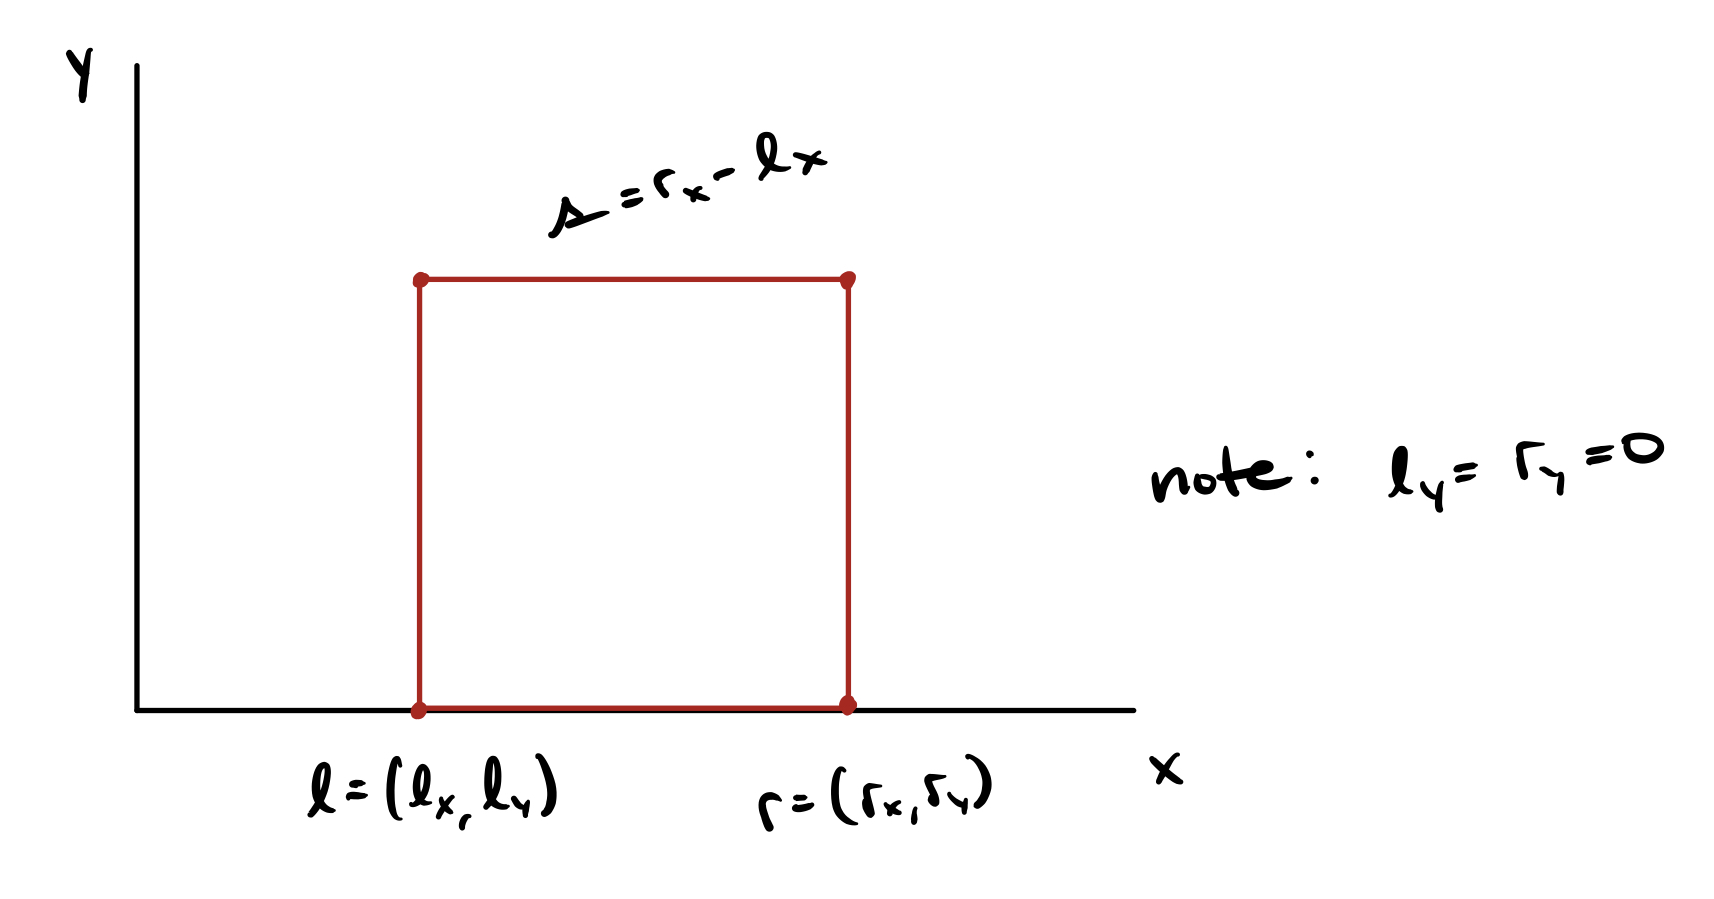
\includegraphics[width=0.65\textwidth]{square}
        \label{fig:square}
        \caption{Annotating the square}
    \end{figure}

    \newpage
    For the runtime, the reduction is merely an $O(1)$ operation on $n$ items for a total of $O(n)$ time.
    Then the linear program will take expected $O(n)$ time since there will be $2n$ constraints.
    Thus the algorithm will take $O(n)$ expected linear time.

\end{enumerate}

\end{document}
